\subsection{Exogenous IFIT1, IFIT3, and IFIT5 Localisation  During RSV Infection} \label{subsec:Exogenous IFIT1, IFIT3, and IFIT5 Localisation  During RSV Infection}
\subsubsection{OE IFIT1}
Overexpressed hIFIT1-FLAG colocalises with both human and bovine RSV IBs. This data is supported by evidence from z stacks.

\begin{figure}
    \begin{subfigure}{0.495\textwidth}
        \caption{}
        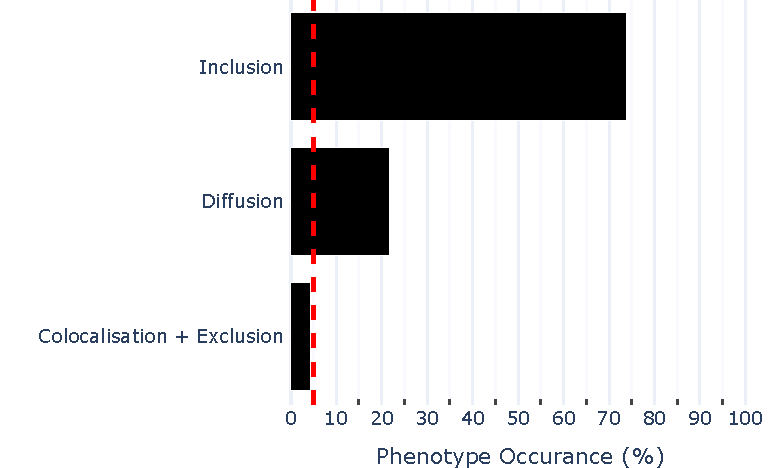
\includegraphics[width=1\linewidth]{09. Chapter 4/Figs/04. Overexpression/01. IFIT1/01. bar_i1_hrsv.pdf} 
    \end{subfigure}
    \begin{subfigure}{0.495\textwidth}
        \caption{}
        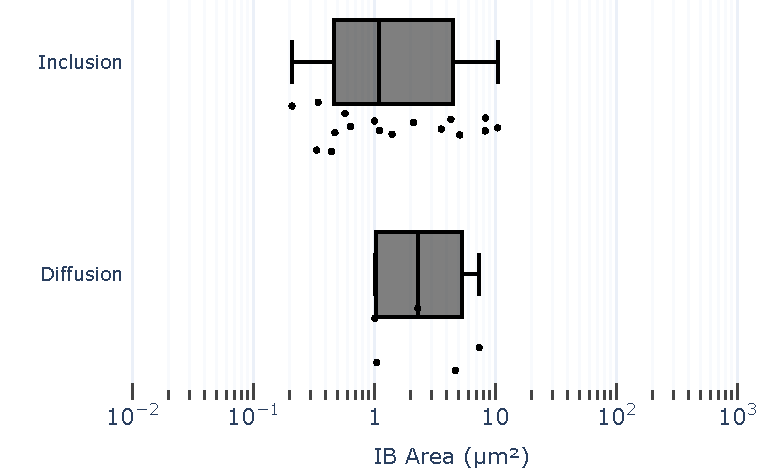
\includegraphics[width=1\linewidth]{09. Chapter 4/Figs/04. Overexpression/01. IFIT1/02. box_i1_hrsv.pdf}
    \end{subfigure}
    \caption[Phenotypic Diversity of Exogenous hIFIT1 Interactions with hRSV Inclusion Bodies in VERO Cell Line.]{\textbf{Phenotypic Diversity of Exogenous hIFIT1 Interactions with hRSV Inclusion Bodies in VERO Cell Line.} 23}
    \label{fig:Phenotypic Diversity of Exogenous hIFIT1 Interactions with hRSV Inclusion Bodies in VERO Cell Line}
\end{figure}

\begin{figure}
    \centering
    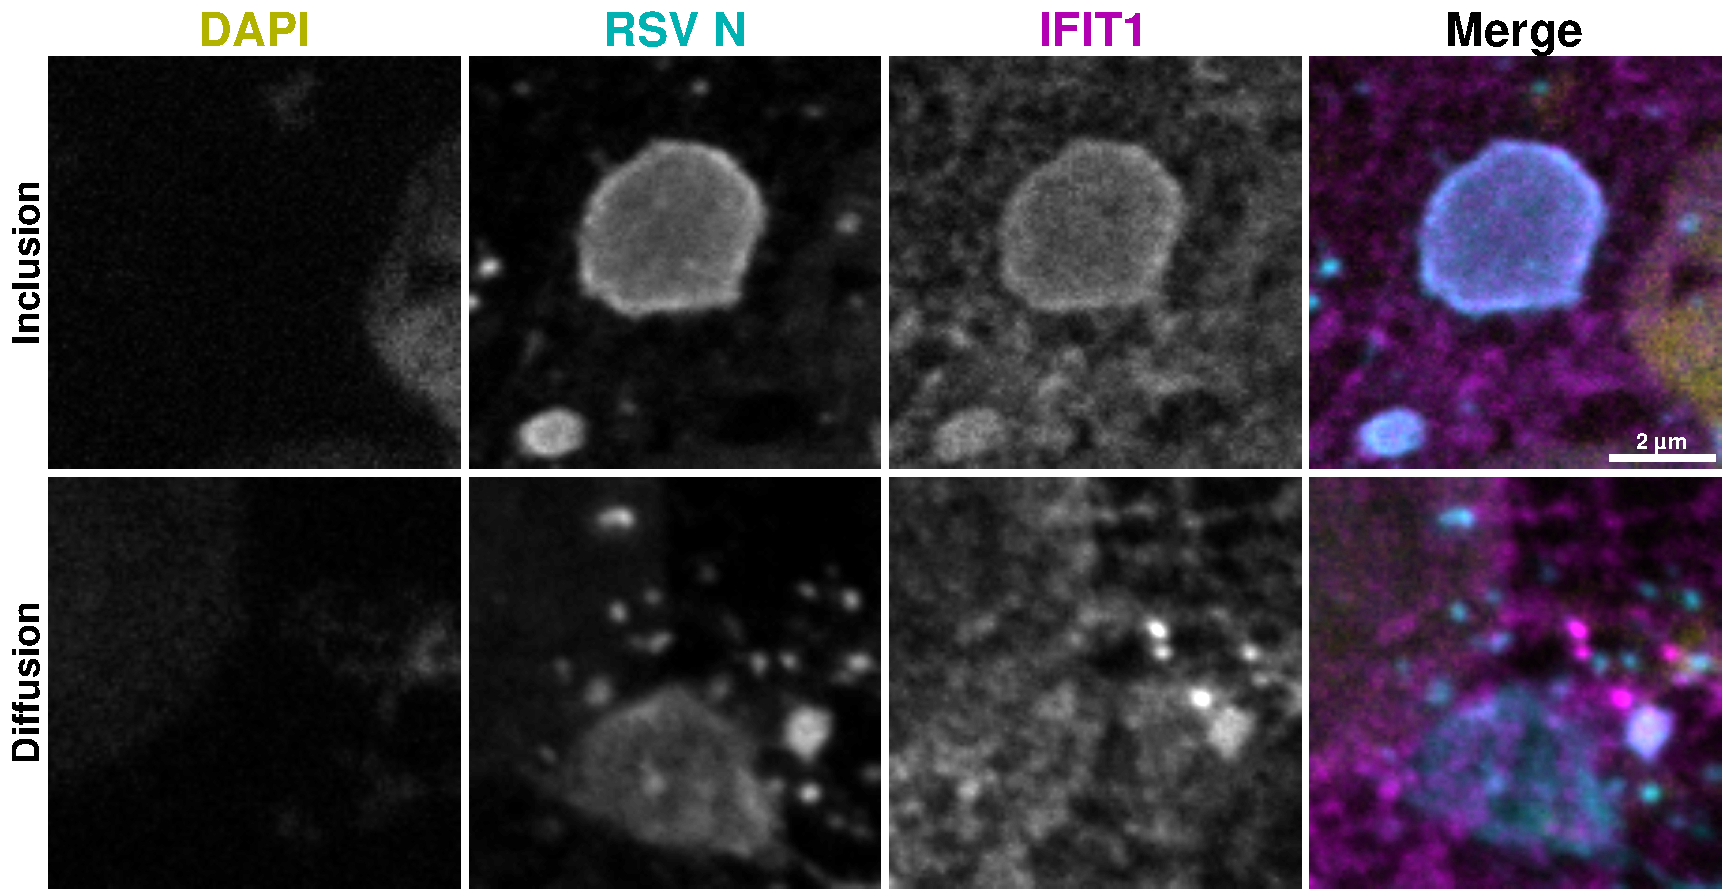
\includegraphics[width=1\linewidth]{09. Chapter 4/Figs/04. Overexpression/01. IFIT1/03. i1-hrsv.pdf}
    \caption[Representative Images of Phenotypic Diversity of Exogenous hIFIT1 Interactions with hRSV Inclusion Bodies in VERO Cell Line.]{\textbf{Representative Images of Phenotypic Diversity of Exogenous hIFIT1 Interactions with hRSV Inclusion Bodies in VERO Cell Line.} }
    \label{fig:Representative Images of Phenotypic Diversity of Exogenous hIFIT1 Interactions with hRSV Inclusion Bodies in VERO Cell Line}
\end{figure}


\begin{figure}
    \begin{subfigure}{0.495\textwidth}
        \caption{}
        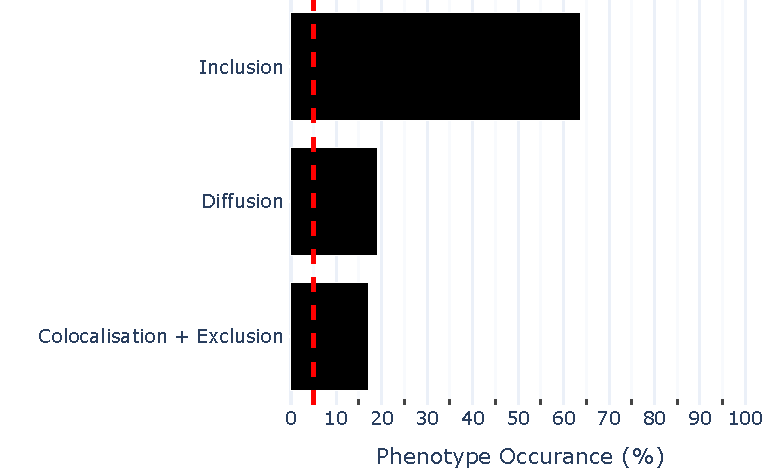
\includegraphics[width=1\linewidth]{09. Chapter 4/Figs/04. Overexpression/01. IFIT1/04. bar_i1_brsv.pdf} 
    \end{subfigure}
    \begin{subfigure}{0.495\textwidth}
        \caption{}
        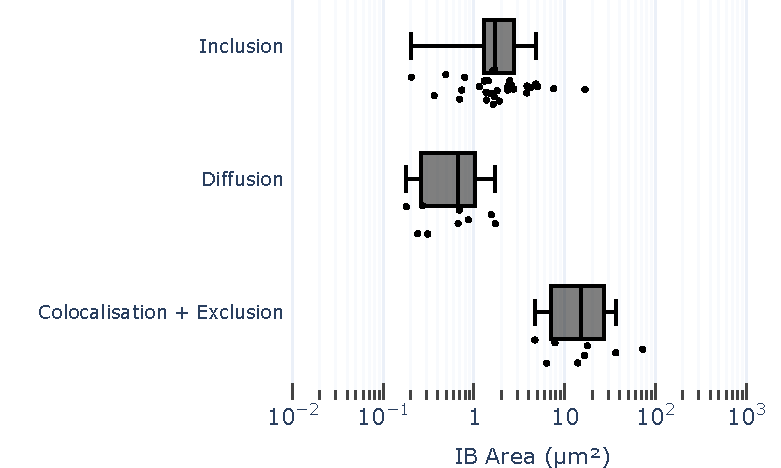
\includegraphics[width=1\linewidth]{09. Chapter 4/Figs/04. Overexpression/01. IFIT1/05. box_i1_brsv.pdf}
    \end{subfigure}
    \caption[Phenotypic Diversity of Exogenous hIFIT1 Interactions with bRSV Inclusion Bodies in VERO Cell Line.]{\textbf{Phenotypic Diversity of Exogenous hIFIT1 Interactions with bRSV Inclusion Bodies in VERO Cell Line.} 47}
    \label{fig:Phenotypic Diversity of Exogenous hIFIT1 Interactions with bRSV Inclusion Bodies in VERO Cell Line}
\end{figure}

\begin{figure}
    \centering
    \includegraphics[width=1\linewidth]{09. Chapter 4/Figs/04. Overexpression/01. IFIT1/06. i1-brsv.pdf}
    \caption[Representative Images of Phenotypic Diversity of Exogenous hIFIT1 Interactions with bRSV Inclusion Bodies in VERO Cell Line.]{\textbf{Representative Images of Phenotypic Diversity of Exogenous hIFIT1 Interactions with bRSV Inclusion Bodies in VERO Cell Line.} }
    \label{fig:Representative Images of Phenotypic Diversity of Exogenous hIFIT1 Interactions with bRSV Inclusion Bodies in VERO Cell Line}
\end{figure}


\subsubsection{OE IFIT3}
Overexpressed bIFIT3-FLAG was observed to colocalise with hRSV inclusion bodies (top panel; highlighted with arrows), as well as being excluded from the hRSV IBs, without any signs of IFIT3 signal on the periphery of the IB structures (middle and bottom panel). This data is supported by z stack measurements.

\begin{figure}
    \begin{subfigure}{0.495\textwidth}
        \caption{}
        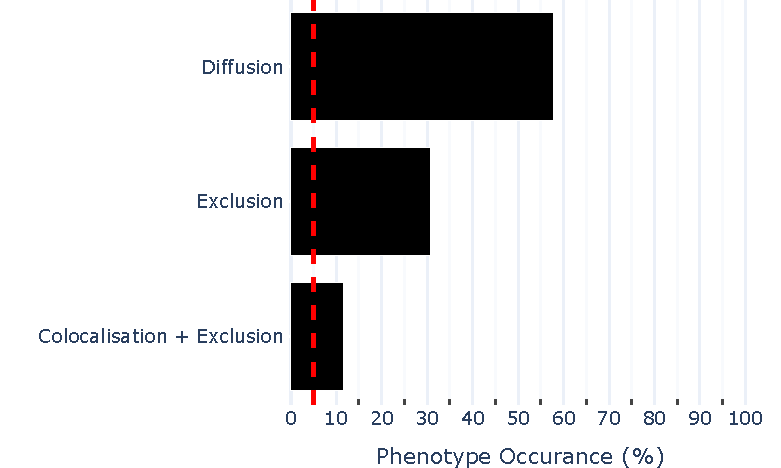
\includegraphics[width=1\linewidth]{09. Chapter 4/Figs/04. Overexpression/02. IFIT3/01. bar_i3_hrsv.pdf} 
    \end{subfigure}
    \begin{subfigure}{0.495\textwidth}
        \caption{}
        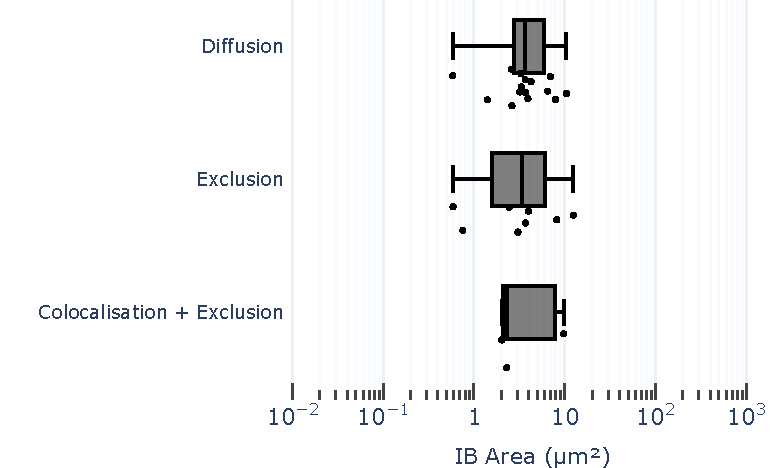
\includegraphics[width=1\linewidth]{09. Chapter 4/Figs/04. Overexpression/02. IFIT3/02. box_i3_hrsv.pdf}
    \end{subfigure}
    \caption[Phenotypic Diversity of Exogenous bIFIT3 Interactions with hRSV Inclusion Bodies in VERO Cell Line.]{\textbf{Phenotypic Diversity of Exogenous bIFIT3 Interactions with hRSV Inclusion Bodies in VERO Cell Line.} 26}
    \label{fig:Phenotypic Diversity of Exogenous bIFIT3 Interactions with hRSV Inclusion Bodies in VERO Cell Line}
\end{figure}

\begin{figure}
    \centering
    \includegraphics[width=1\linewidth]{09. Chapter 4/Figs/04. Overexpression/02. IFIT3/03. bi3-hrsv.pdf}
    \caption[Representative Images of Phenotypic Diversity of Exogenous bIFIT3 Interactions with hRSV Inclusion Bodies in VERO Cell Line.]{\textbf{Representative Images of Phenotypic Diversity of Exogenous bIFIT3 Interactions with hRSV Inclusion Bodies in VERO Cell Line.} }
    \label{fig:Representative Images of Phenotypic Diversity of Exogenous bIFIT3 Interactions with hRSV Inclusion Bodies in VERO Cell Line}
\end{figure}

Very similar phenotype is observed for overexpressed bIFIT3-FLAG in bRSV infected cells. We see colocalization with IB (top panel) as well as exclusion from the structure without any signs of IFIT3 signal on the periphery of the IB structure (bottom panel). This data is as well supported by z stack measurements.

\begin{figure}
    \begin{subfigure}{0.495\textwidth}
        \caption{}
        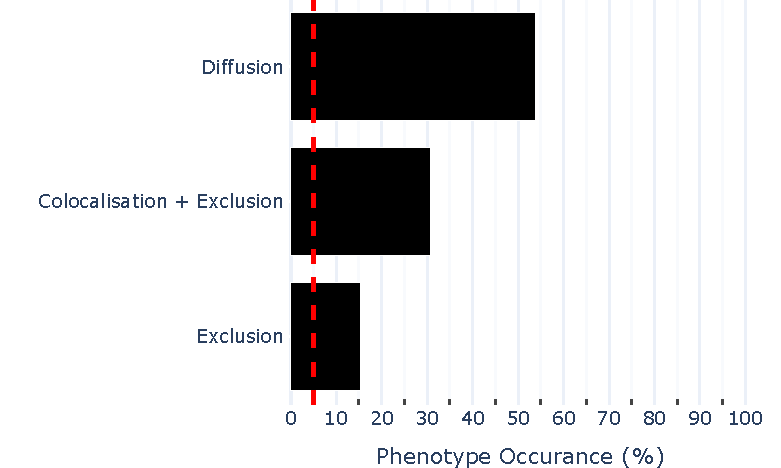
\includegraphics[width=1\linewidth]{09. Chapter 4/Figs/04. Overexpression/02. IFIT3/04. bar_i3_brsv.pdf} 
    \end{subfigure}
    \begin{subfigure}{0.495\textwidth}
        \caption{}
        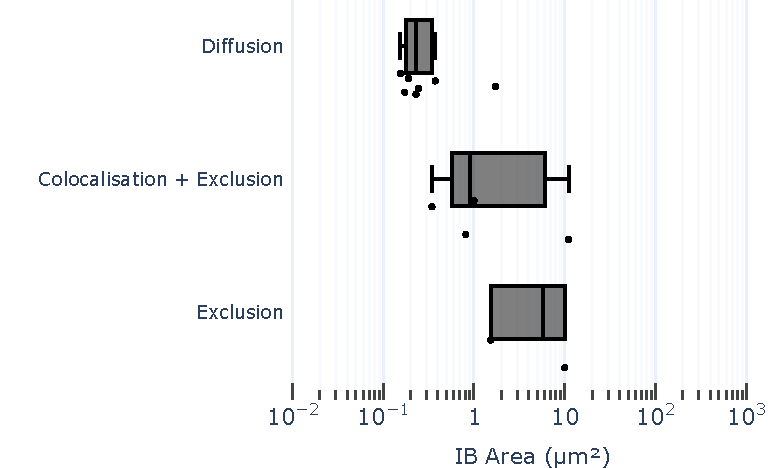
\includegraphics[width=1\linewidth]{09. Chapter 4/Figs/04. Overexpression/02. IFIT3/05. box_i3_brsv.pdf}
    \end{subfigure}
    \caption[Phenotypic Diversity of Exogenous bIFIT3 Interactions with bRSV Inclusion Bodies in VERO Cell Line.]{\textbf{Phenotypic Diversity of Exogenous bIFIT3 Interactions with bRSV Inclusion Bodies in VERO Cell Line.} 13}
    \label{fig:Phenotypic Diversity of Exogenous bIFIT3 Interactions with bRSV Inclusion Bodies in VERO Cell Line}
\end{figure}

\begin{figure}
    \centering
    \includegraphics[width=1\linewidth]{09. Chapter 4/Figs/04. Overexpression/02. IFIT3/06. bi3-brsv.pdf}
    \caption[Representative Images of Phenotypic Diversity of Exogenous bIFIT3 Interactions with bRSV Inclusion Bodies in VERO Cell Line.]{\textbf{Representative Images of Phenotypic Diversity of Exogenous bIFIT3 Interactions with bRSV Inclusion Bodies in VERO Cell Line.} }
    \label{fig:Representative Images of Phenotypic Diversity of Exogenous bIFIT3 Interactions with bRSV Inclusion Bodies in VERO Cell Line}
\end{figure}

\subsubsection{OE IFIT5}
hIFIT5-FLAG is colocalising with hRSV inclusion bodies (basically resembling the P staining), while in bRSV infected cell there is a hint of IFIT5 signal concentration at the side of bRSV IB.

This data is by single cells per conditions as transfection did not work well. It is however supported by z stack measurements.

\begin{figure}
    \begin{subfigure}{0.495\textwidth}
        \caption{}
        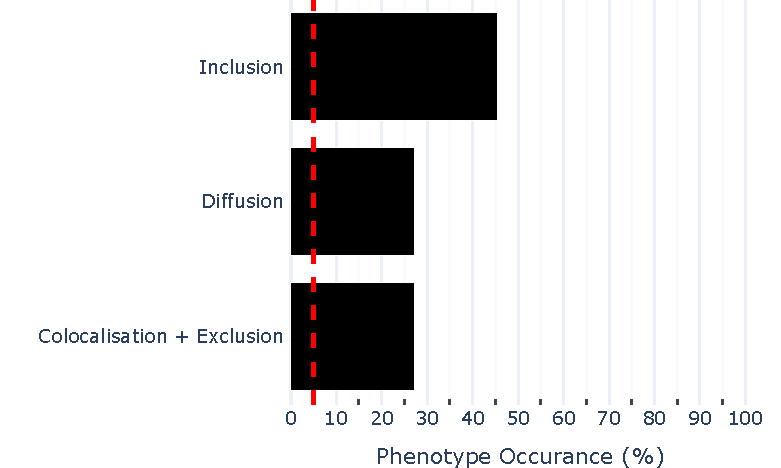
\includegraphics[width=1\linewidth]{09. Chapter 4/Figs/04. Overexpression/03. IFIT5/01. bar_i5_hrsv.pdf} 
    \end{subfigure}
    \begin{subfigure}{0.495\textwidth}
        \caption{}
        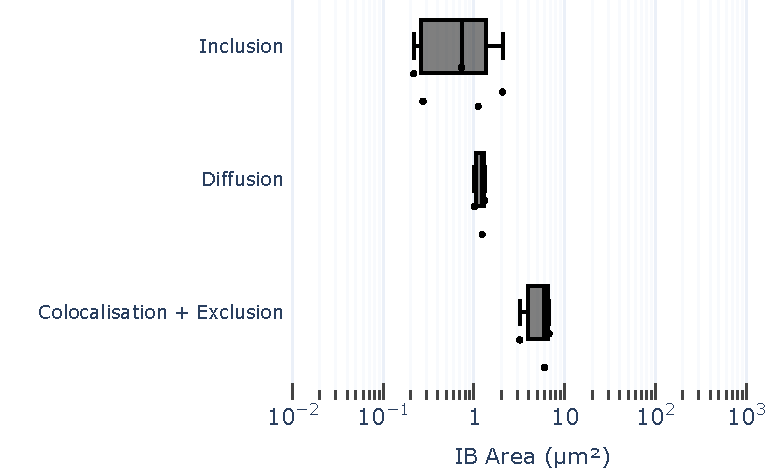
\includegraphics[width=1\linewidth]{09. Chapter 4/Figs/04. Overexpression/03. IFIT5/02. box_i5_hrsv.pdf}
    \end{subfigure}
    \caption[Phenotypic Diversity of Exogenous hIFIT5 Interactions with hRSV Inclusion Bodies in VERO Cell Line.]{\textbf{Phenotypic Diversity of Exogenous hIFIT5 Interactions with hRSV Inclusion Bodies in VERO Cell Line.} 11}
    \label{fig:Phenotypic Diversity of Exogenous hIFIT5 Interactions with hRSV Inclusion Bodies in VERO Cell Line}
\end{figure}

\begin{figure}
    \centering
    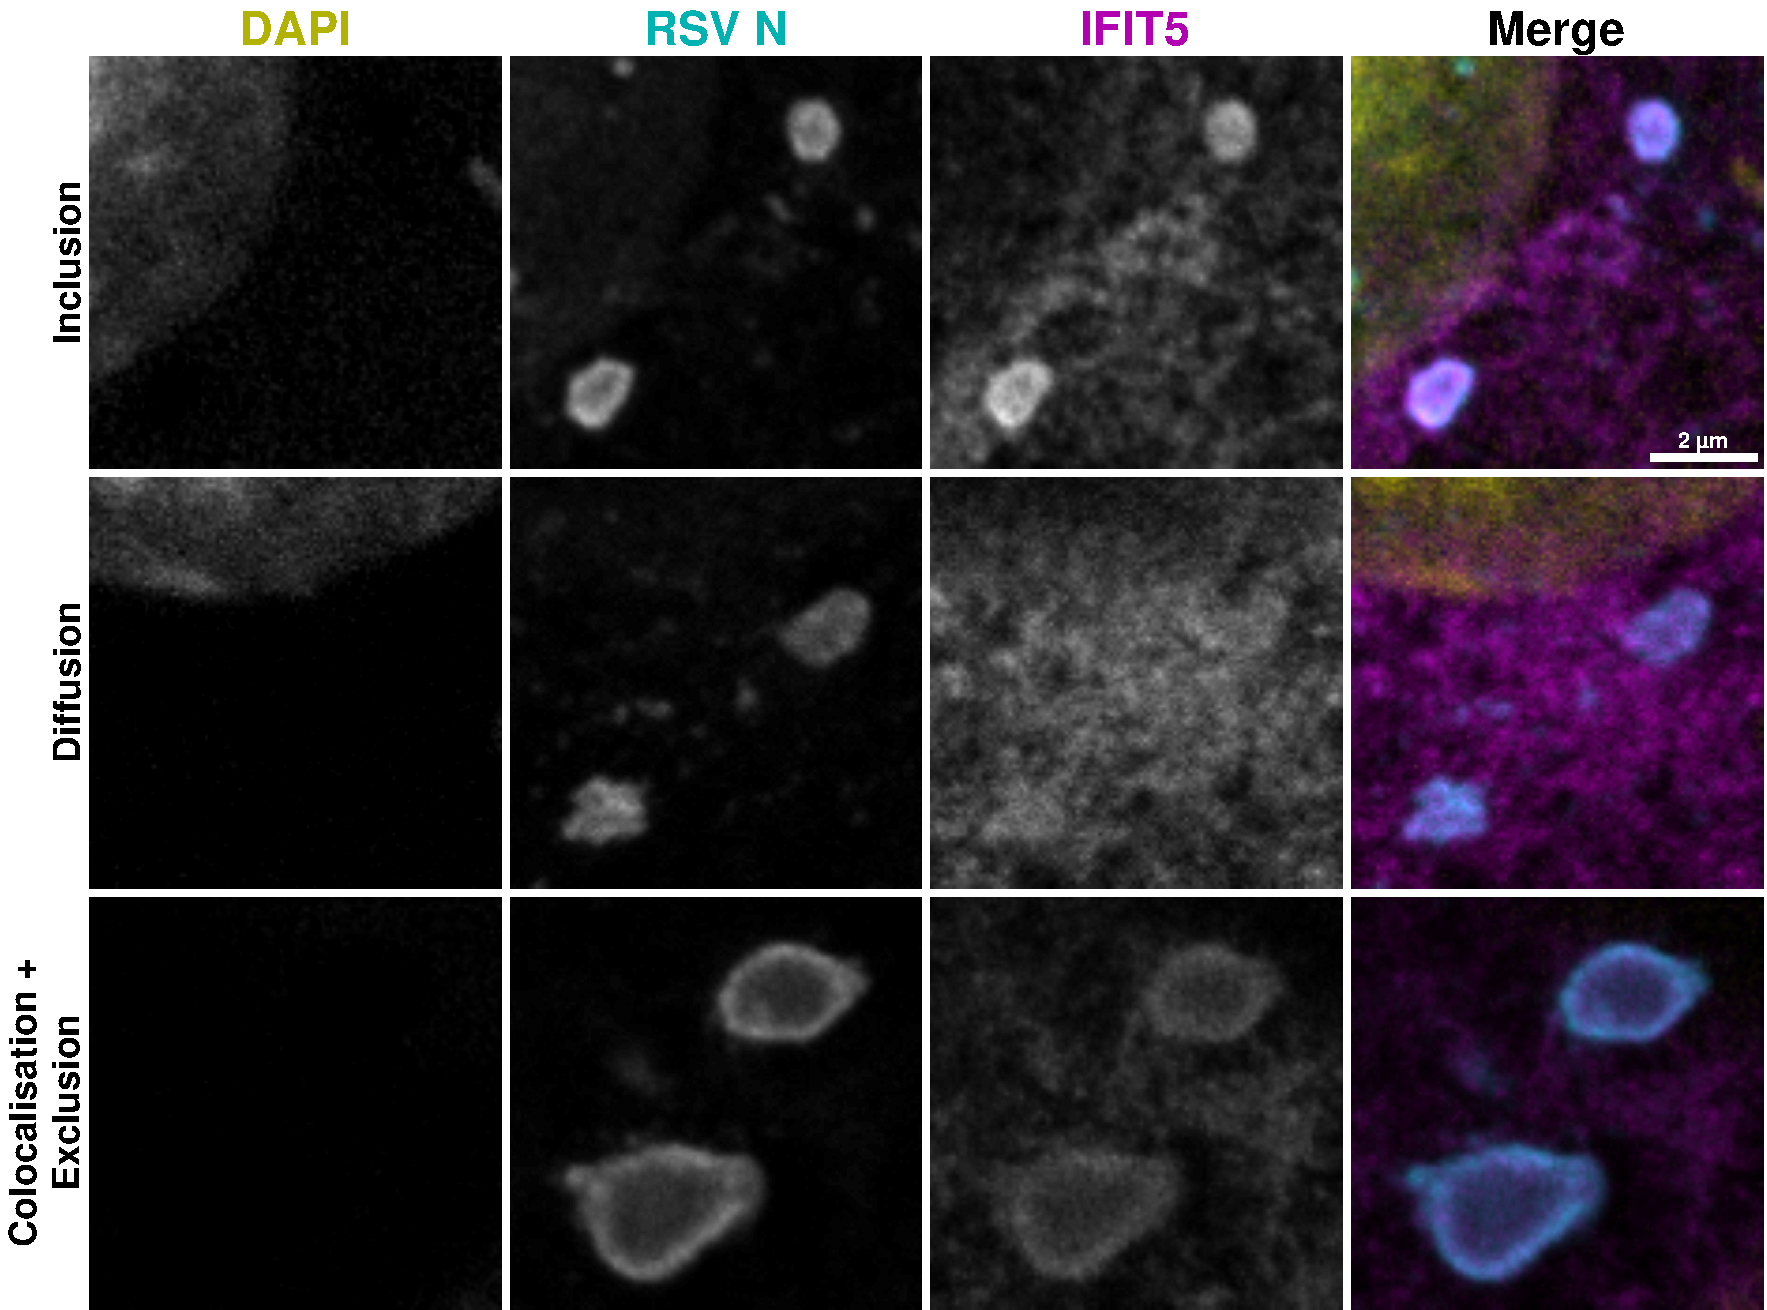
\includegraphics[width=1\linewidth]{09. Chapter 4/Figs/04. Overexpression/03. IFIT5/03. i5-hrsv.pdf}
    \caption[Representative Images of Phenotypic Diversity of Exogenous hIFIT5 Interactions with hRSV Inclusion Bodies in VERO Cell Line.]{\textbf{Representative Images of Phenotypic Diversity of Exogenous hIFIT5 Interactions with hRSV Inclusion Bodies in VERO Cell Line.} }
    \label{fig:Representative Images of Phenotypic Diversity of Exogenous hIFIT5 Interactions with hRSV Inclusion Bodies in VERO Cell Line}
\end{figure}

\begin{figure}
    \begin{subfigure}{0.495\textwidth}
        \caption{}
        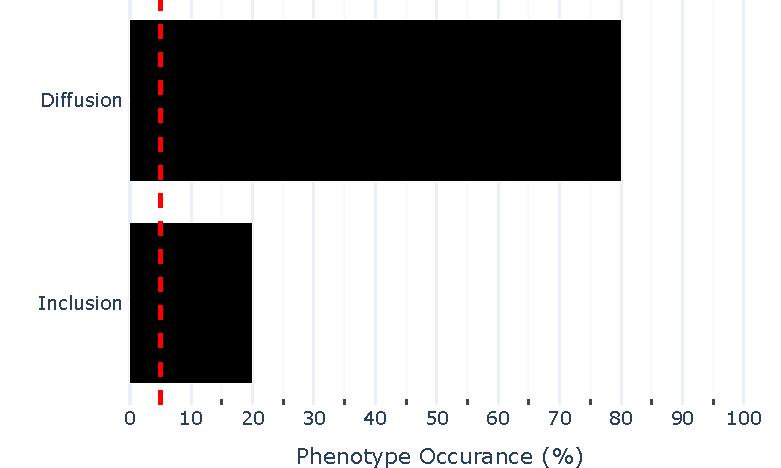
\includegraphics[width=1\linewidth]{09. Chapter 4/Figs/04. Overexpression/03. IFIT5/04. bar_i5_brsv.pdf} 
    \end{subfigure}
    \begin{subfigure}{0.495\textwidth}
        \caption{}
        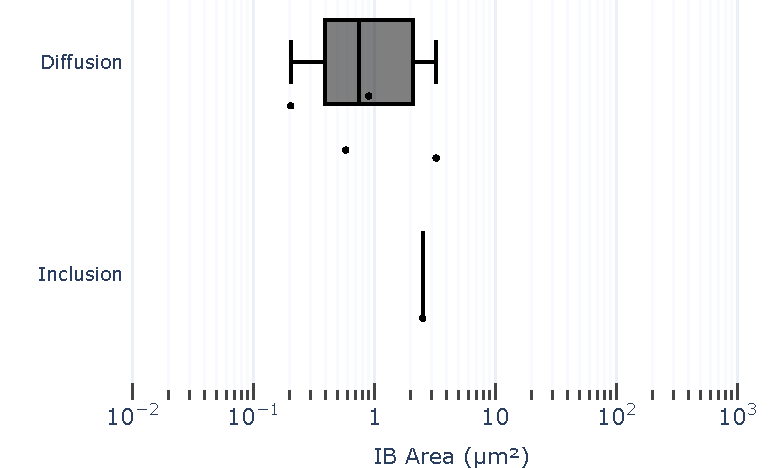
\includegraphics[width=1\linewidth]{09. Chapter 4/Figs/04. Overexpression/03. IFIT5/05. box_i5_brsv.pdf}
    \end{subfigure}
    \caption[Phenotypic Diversity of Exogenous hIFIT5 Interactions with bRSV Inclusion Bodies in VERO Cell Line.]{\textbf{Phenotypic Diversity of Exogenous hIFIT5 Interactions with bRSV Inclusion Bodies in VERO Cell Line.} 5}
    \label{fig:Phenotypic Diversity of Exogenous hIFIT5 Interactions with bRSV Inclusion Bodies in VERO Cell Line}
\end{figure}

\begin{figure}
    \centering
    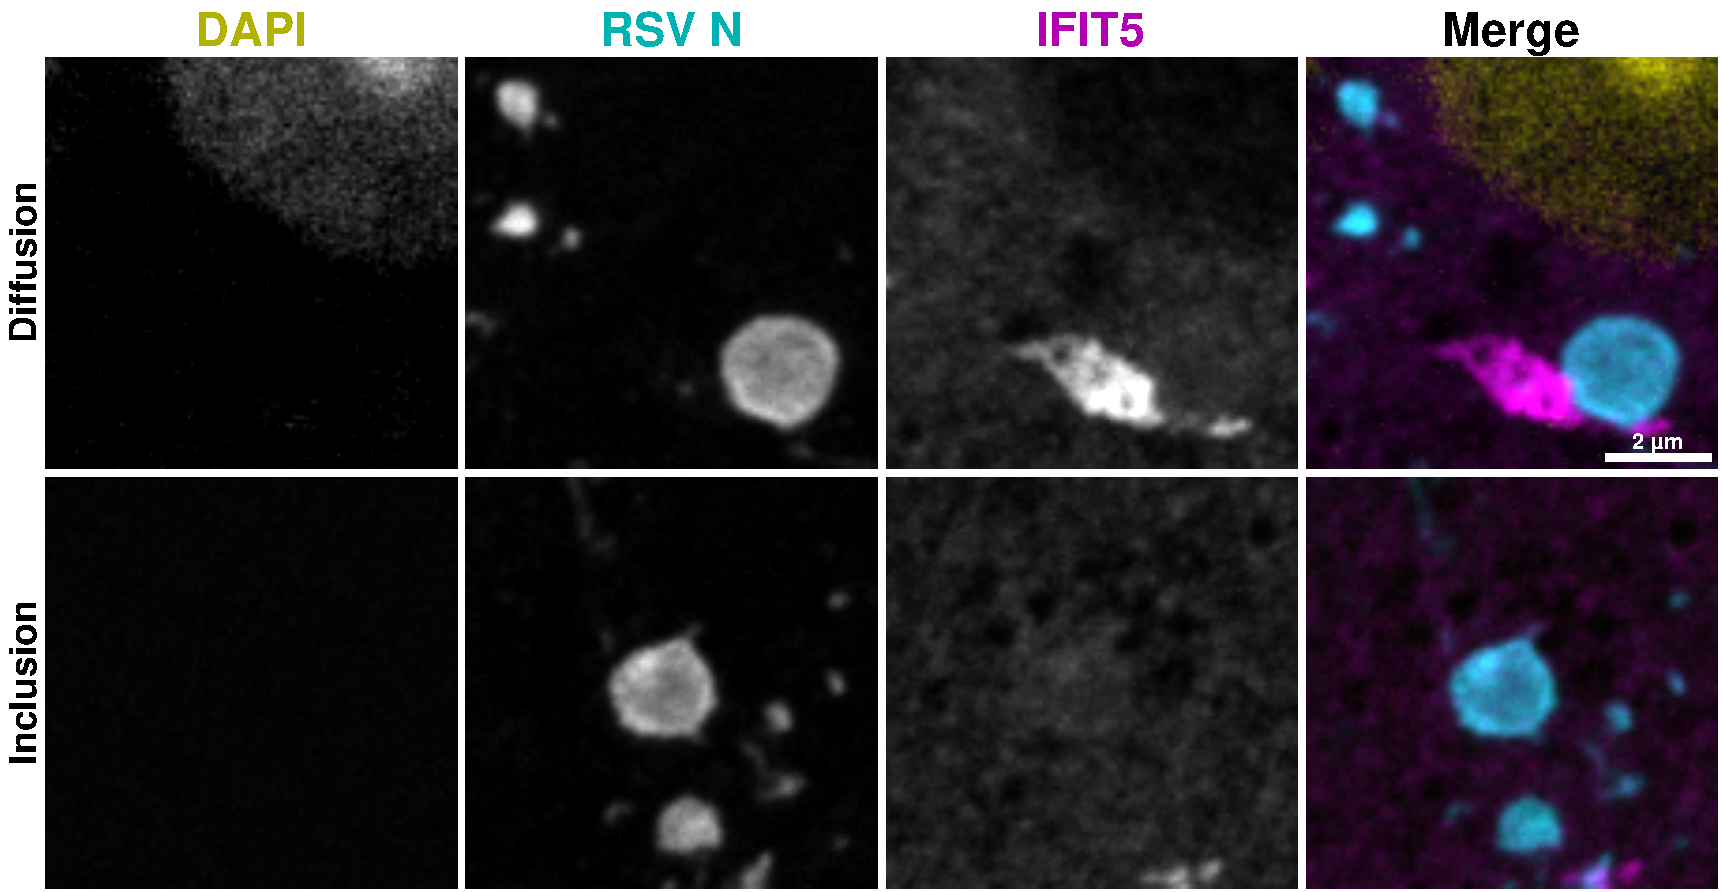
\includegraphics[width=1\linewidth]{09. Chapter 4/Figs/04. Overexpression/03. IFIT5/06. i5-brsv.pdf}
    \caption[Representative Images of Phenotypic Diversity of Exogenous hIFIT5 Interactions with bRSV Inclusion Bodies in VERO Cell Line.]{\textbf{Representative Images of Phenotypic Diversity of Exogenous hIFIT5 Interactions with bRSV Inclusion Bodies in VERO Cell Line.} }
    \label{fig:Representative Images of Phenotypic Diversity of Exogenous hIFIT5 Interactions with bRSV Inclusion Bodies in VERO Cell Line}
\end{figure}

\subsubsection{Summary} \label{Summary-oe}
Overexpressed hIFIT1-FLAG in the context of h/bRSV infection colocalises to both human and bovine IB structures.

Overexpressed bIFIT3 behaves equally between hRSV and bRSV infection, that is it sometimes colocalises with the IB structure and sometimes is completely excluded from the structure.

Overexpressed hIFIT5 in hRSV infected cells colocalises with the IBs.